% Chapter Template

\chapter{Work Environment} % Main chapter title

\label{Chapter2} % Change X to a consecutive number; for referencing this chapter elsewhere, use \ref{ChapterX}


%----------------------------------------------------------------------------------------
%	INTRODUCTION
%----------------------------------------------------------------------------------------

\section*{Introduction}

This chapter presents in general terms the work environment and the goals of the student's end-of-study project.

It will start by a presentation of the host organization, Bang\&Olufsen, then the department where the student worked and finally expound a short exploration brief on the internship itself.   

%----------------------------------------------------------------------------------------
%	SECTION 1
%----------------------------------------------------------------------------------------

\section{Bang \& Olufsen}

%-----------------------------------
%	SUBSECTION 1
%-----------------------------------
\subsection{The Company}

Founded in 1925 by Peter Bang and Svend Olufsen in Struer, Denmark, the company initially started by selling radio devices plugged to an outlet and thus functioning with alternating current. Compared to the other kind of equipments at that time, that were working on battery and therefore expensive and impractical, their inventions became a life-changer for a lot of people and were the beginnings of their success. 

Nowadays, Bang \& Olufsen is well-known worldwide as a luxury brand for its distinctive design, sound quality and innovative technology of its products. The current portfolio includes:
\begin{itemize}
	\item Wireless speaker systems (Beosound Shape, Beosound 2, \dots).
	\item Televisions (Beovision Eclipse, Beovision Avant, \dots).
	\item Speakers (Beolab Collection, \dots).
	\item Portable bluetooth speakers (Beoplay A1, Beolit 17, \dots).
	\item Sound systems (Beosound Core).
\end{itemize}

The company headquarters are still in Struer, where part of the development and the production also takes place. The other production facility is located in the Czech Republic, mainly focused on assembly and quality testing. The company site in Copenhagen deals with global sales and the \href{https://www.beoplay.com/en}{B\&O PLAY} brand section as well as some software development. Recently, Bang \& Olufsen sold its automotive business to \href{https://www.harman.com}{HARMAN}, but it collaborates with \href{https://www8.hp.com/us/en/home.html}{Hewlett-Packard} to bring the B\&O sound to HP’s products, and it also has a recent partnership with \href{https://www.lg.com/us}{LG Electronics} on TVs and audio solutions for smartphones.

\newpage
%The organisational chart of the compagny is presented in Figure \ref{Figure 2.1} infra. It can be seen that the COO area, whose role is to ensure efficiency and effectiveness of the business operations, is on top of the structure. Then we have five group functions (Portfolio \& Program Management, Transformation, Group Operation, Group Quality \& Service, and Group System Management), the Finance, and finally the Human Resources. The five business units where the company focuses are: Vision, Advanced Sound, Premium Sound, Smart Home, and Interaction. The three platforms that supports them are: Platform Development, Research, Maintenance; Cloud computing and Applications; Design, UX \& Concept Exploration.
%
%
%\begin{figure}[!htb]
%	\begin{center}
%		\begin{minipage}{1.2\textwidth}
%			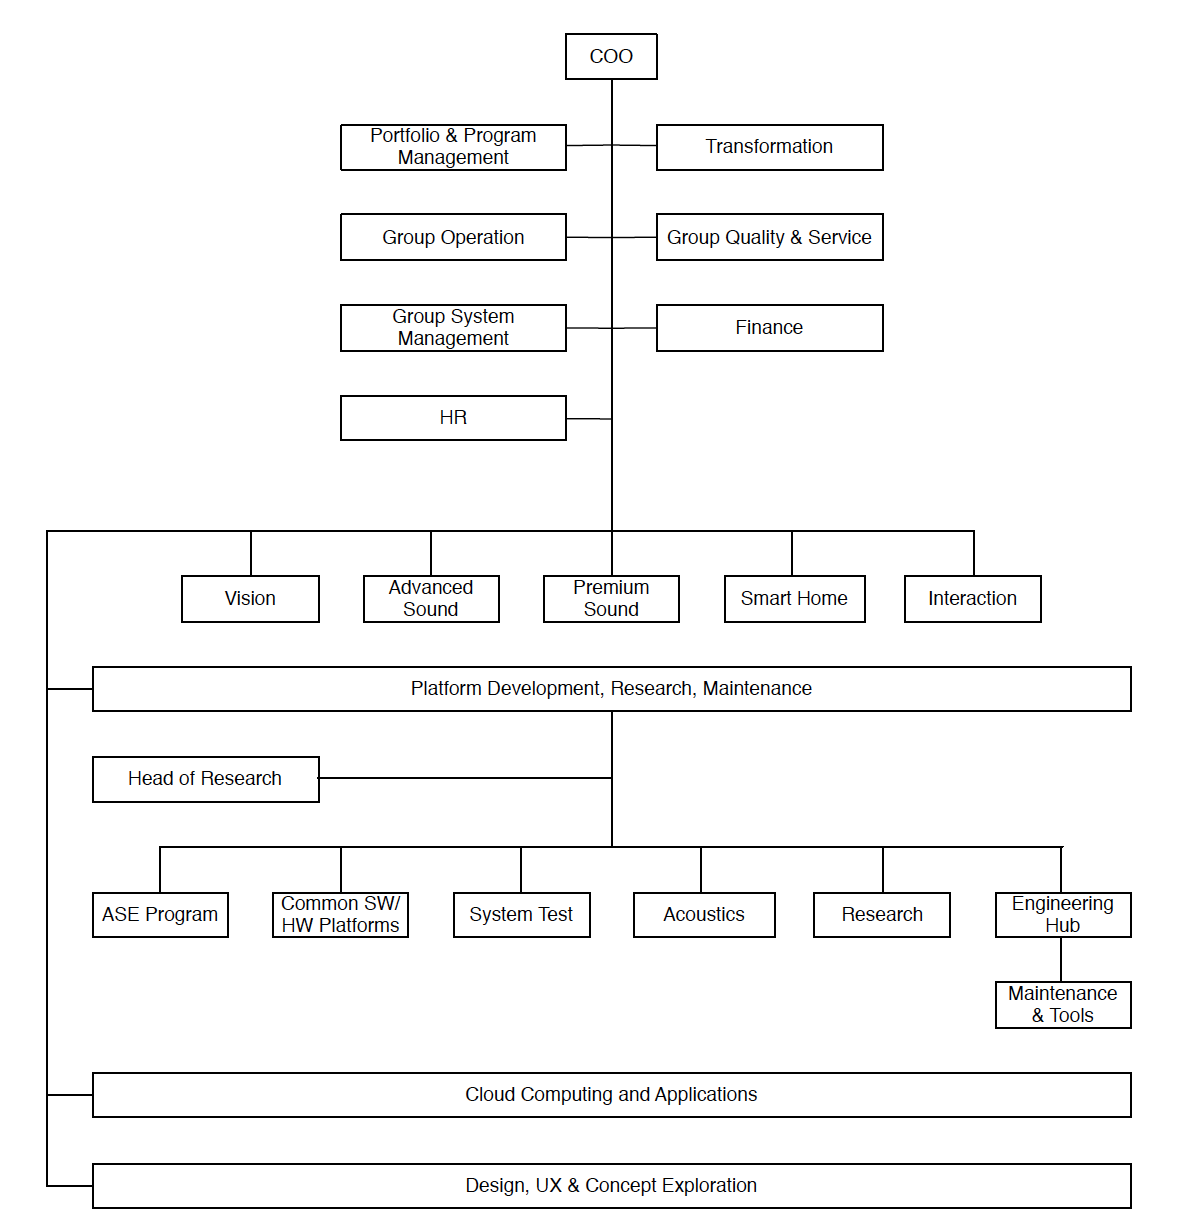
\includegraphics[width=0.87 \linewidth]{orga.png}
%			\caption{Organisational Chart of Bang \& Olufsen}\label{Figure 2.1}
%		\end{minipage}\hfill
%	\end{center}	
%\end{figure}

%-----------------------------------
%	SUBSECTION 2
%-----------------------------------

\newpage
\subsection{R\&D Acoustics}
The student worked in the research department, which is under the Platform Development, Research, Maintenance section. The responsibilities of this department are:
\begin{itemize}
	\item Establish, implement and maintain research strategy to support product roadmap.
	\item Internal communication and alignment with key stakeholders.
	\item Write, coordinate and track funding applications.
	\item Initiate and support patent process.
	\item Establish and maintain collaboration with external partners (universities, companies).
	\item Represent B\&O in relevant funding bodies and committees.
\end{itemize}

In the figure below, the current (during the time of the internship) organization of the Acoustics \& Research department is shown. It is divided into five parts: Research, Sound Quality \& Design, Electro Acoustics, Acoustic Test \& Validation, and Acoustic \hyperlink{DSP}{DSP}.

\begin{figure}[ht!]
		\centering
		%\begin{minipage}{1.2\textwidth}
			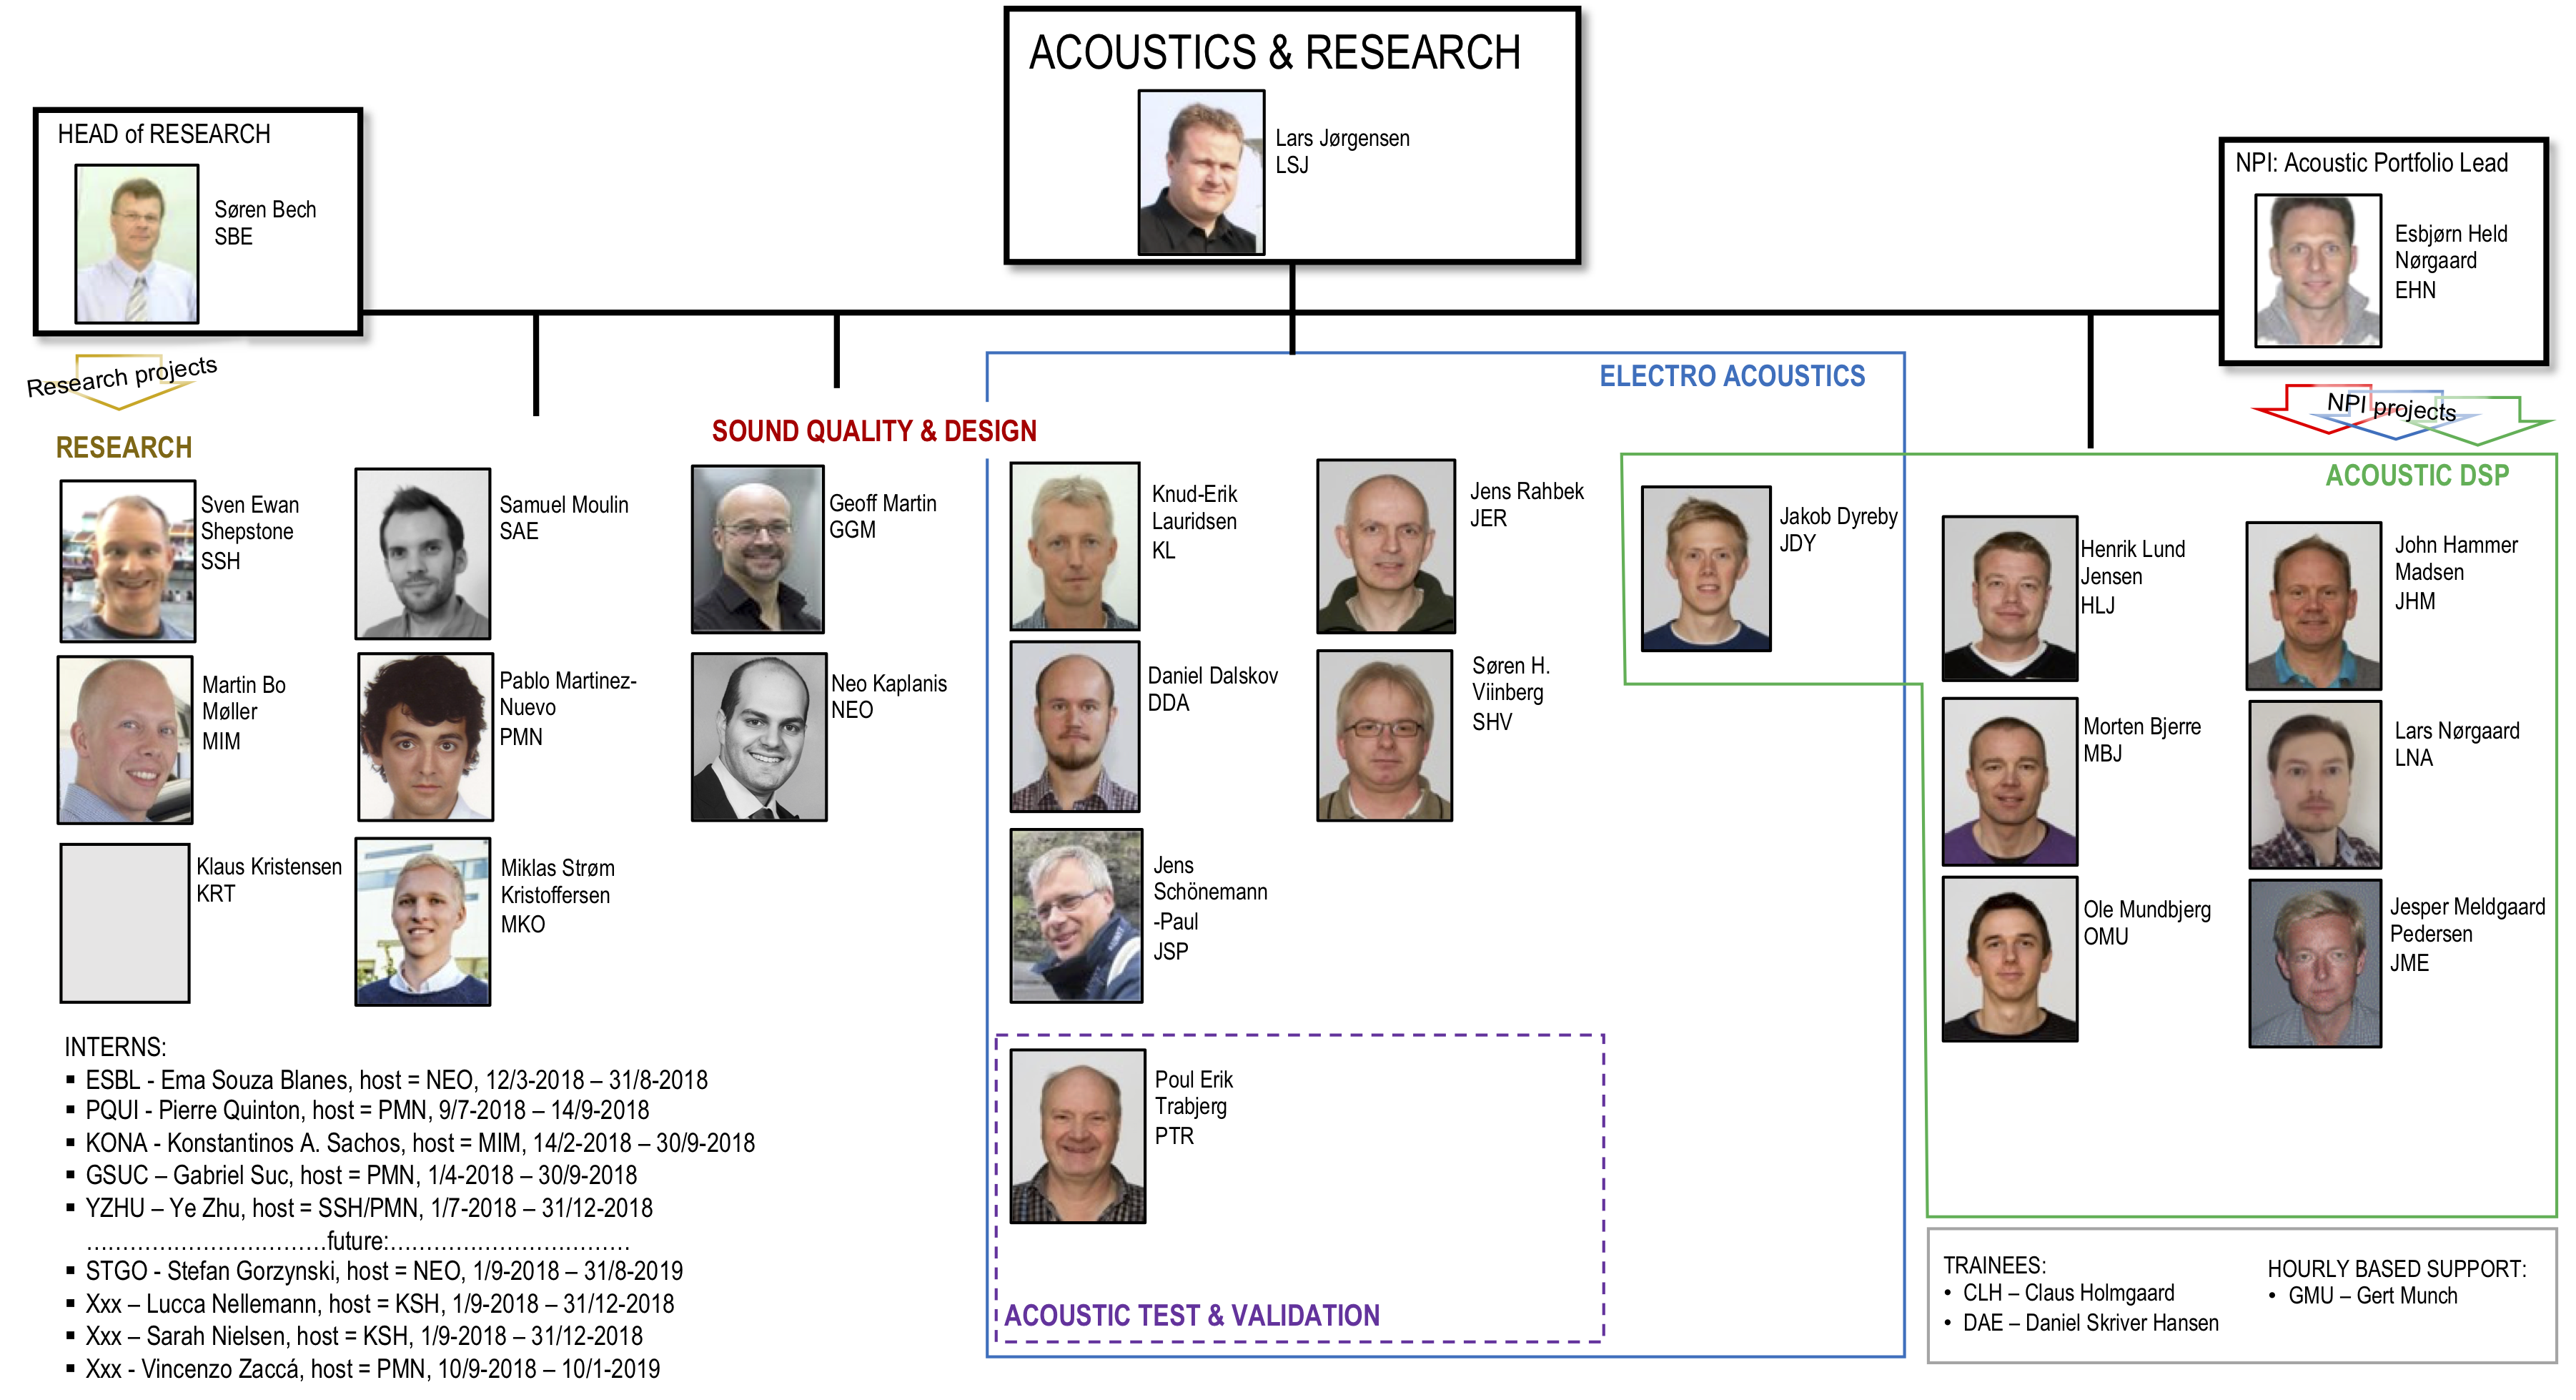
\includegraphics[scale =0.25]{research.png}
			\caption{Organization Chart of the Acoustics \& Research Department}\label{Figure 2.2}
		%\end{minipage}\hfill

\end{figure}

The internship was mainly supervised by Dr. Pablo Martínez-Nuevo, providing precious help and directives on the design and implementation of the \hyperlink{DSP}{DSP} algorithm. Dr. Sven Ewan Shepstone gave essential input on the matter and assisted the student on the software implementation facet. Finally, Mr. Henrik Lund Jensen and Mr. Geoff Martin lent their support for the design and the implementation of the algorithm as well as establishing a performance evaluation and a set of requirements.
%----------------------------------------------------------------------------------------
%	SECTION 2
%----------------------------------------------------------------------------------------

\newpage

%----------------------------------------------------------------------------------------
%	SECTION 3
%----------------------------------------------------------------------------------------

\section{Exploration Brief}

This section is here to define properly what the project was about and the context in which it happened. Moreover, a time structure will also be provided.\\

The goal of the project was to design and implement a sample rate converter that meets the quality and computational demands of a real-time audio signal processing chain and that can be integrated in future and current software platforms. Modern audio/visual devices consist of several sub-systems operating at different rates. Sampling rate conversion is the key operation that makes these blocks working together. Despite being a crucial, and widely used operation of many discrete-time processing systems, it has been broadly overlooked, often resulting in poor performance. 

On one hand, open-source software implementations of sampling rate conversion used in Bang \& Olufsen products (e.g. GStreamer) create audible artifacts that do not meet the performance standards of B\&O audio quality. On the other hand, third-party proprietary implementations (e.g. Audio-Weaver) do not provide full support for the variety of sampling rates that are required in B\&O systems. Moreover, since there is no control over its design and implementation, it is not viable to reliably evaluate and accommodate its performances to the company's needs.

Therefore, this project aims at establishing the design criteria of a sampling rate converter as well as providing a computationally efficient implementation that meets the appropriate quality demands. \\

The project had to explore certain points that, with the different constraints and limitations, served as guidelines: 

\begin{itemize}
	\item The impact on audio quality of the implementation of sample-rate conversion systems in GStreamer that are currently used by B\&O products. 
	\item Review the design criteria and implementation of available open-source sample rate converters.
	\item Establish the criteria for an appropriate performance in terms of filter design taking into account perceptual aspects. 
	\item Explore the different tradeoffs for implementation that may involve throughput, latency, real-time operation, CPU and memory usage, or power consumption. 
	\item Evaluate the performance of different approaches to perform linear convolution in an efficient manner.
	\item Design the sample-rate converter considering the knowledge gathered from the previous stages and considering the synchronous and asynchronous approaches.
	\item Implement the algorithm in C language and test the performances in different hardware platforms, for instance, ARM-based processors.
	
 
\end{itemize}

However, the student and the supervisors agreed that synchronous sampling rate conversion should be the principal focus for this project, knowing that the asynchronous part was already in the center of other research projects.

Subsequently, the project team had to set a desired planning in order to fulfill the requirements specified above. The initial schedule was as follows, with some modifications that happened along the way: 

\begin{itemize}
	\item \bm{$1^{st}$} \textbf{month:} Study of sample-rate conversion systems and current approaches for implementation.
	\item \bm{$2^{nd}$} \textbf{month:} Formulate a set of requirements for the design of a sample-rate conversion system tailored to  B\&O's needs.
	\item \bm{$3^{rd} - 4^{th}$} \textbf{month:} Implement a C prototype and benchmark.
	\item \bm{$5^{th}$} \textbf{month:} Turn the implementation into a GStreamer plugin.
	\item \bm{$6^{th}$} \textbf{month:} Wrap-up and conclusion. 
\end{itemize}


%----------------------------------------------------------------------------------------
%	CONCLUSION
%----------------------------------------------------------------------------------------

\section*{Conclusion}

As described in this chapter, we are from this point forward aware of the framework of the project. The next part will explain in detail the theoretical background needed to fully grasp the topic of the internship. 
